\section{Concatenation of paths, associativity , unitality}
20.02

\begin{definition}
    Fernando notation:
    \[
      X(x_0, x_1) = \hom_{\text{Top}}^{x_0,x_1}(I, X) / \simeq_p
    \]
\end{definition}


\begin{example}
    \( \mathbb{R}^n(x_0, x_1) = * \).
\end{example}

\begin{definition}[loop]
    A loop is a path from \( x \) to \( x \).
\end{definition}

\begin{definition}[path concatination]
   Let \( f, g: I \to X \) be paths from
   \( x_0  \) to \( x_1 \) and from \( x_1 \)
   to \( x_2 \) respectivly.
   Define the concatination of \( f \) and \( g \) as:
  \begin{equation}
      (g * f)(s) = \begin{cases}
          f(2s) & 0 \le s \le 1/2 \\
          g(2s - 1) & 1/2 \le s \le 1
      \end{cases}
  \end{equation}
\end{definition}

\begin{proposition}
    Path concatination is a well defined operation
    on path homotopy equivalence classes. That is:
    \begin{align*}
      X(x_0,x_1) \times X(x_1, x_2) &\longrightarrow X(x_0, x_2) \\
      ([f], [g]) &\longmapsto [g * f]
    \end{align*}
    is well defined.
\end{proposition}

\begin{proof}
  Let \( f, f': I \to X \) be path homotopic maps
    from \( x_0 \) to \( x_1 \).
  Let \( g, g': I \to X \) be path homotopic maps
    from \( x_1 \) to \( x_2 \).
  Hence, \( f, f' \in [f] \) and \( g, g' \in [g] \).
  We need to show that
    \[
      g * f \simeq_p g' * f'.
    \]
  Let \( H_1 \) be a path homotopy of \( f \) and \( f' \).
  Let \( H_2 \) be a path homotopy of \( g \) and \( g' \).
  Define
  \[
    H_3(t, s) = \begin{cases}
      H_1(t, 2s) & 0 \le s \le 1/2 \\
      H_2(t, 2s -1) & 1/2 \le s \le 1
    \end{cases}
  \]
  \( H_3 \) is well defined since
  \[
    H_3(t, 1/2) = \begin{cases}
      H_1(t, 1) \\
      H_2(t, 0) 
    \end{cases}
    = \begin{cases}
        x_1 \\ x_1
    \end{cases}
    = x_1
  \]
  Check that \( H_3 \) is a path homotopy of 
  \( g * f \) and \( g' * f' \).
  \begin{enumerate}
    \item 
      \begin{align*}
        H_3(0, s) &= \begin{cases}
          H_1(0, 2s) & 0 \le s \le 1/2 \\
          H_2(0, 2s -1) & 1/2 \le s \le 1
          \end{cases} \\
                  &= \begin{cases}
          f(2s) & 0 \le s \le 1/2 \\
          g(2s - 1) & 1/2 \le s \le 1
        \end{cases} \\
                  &= (g * f) (s)
      \end{align*}

    \item 
      \begin{align*}
        H_3(1, s) &= \begin{cases}
          H_1(1, 2s) & 0 \le s \le 1/2 \\
          H_2(1, 2s -1) & 1/2 \le s \le 1
          \end{cases} \\
                  &= \begin{cases}
          f'(2s) & 0 \le s \le 1/2 \\
          g'(2s - 1) & 1/2 \le s \le 1
        \end{cases} \\
                  &= (g' * f') (s)
      \end{align*}
  \end{enumerate}
\end{proof}

Notation: Only \( f \) might be used 
instead of \( [f] \) for the equivalence class.

\begin{theorem}
    The operation of concatination
    enjoys the following properties:
    \begin{enumerate}
      \item[1)] Associativity.
        \[
          (h * g) * f \simeq_p h * (g * f)
        \]
      \item[2)] Left/right units.
        \[
          f * c_x \simeq_p f \simeq_p c_y * f
        \]
      \item[3)] Left/right inverses.
        \[
          f * \overline{f} \simeq_p c_y, \overline{f} * f  \simeq_p c_x
        \]
    \end{enumerate}
\end{theorem}

\begin{proof}
  We show the three properties.
  \begin{enumerate}
    \item Associativity.
      Let \( f \in X(x_0, x_1), g \in X(x_1, x_2), h \in X(x_2, x_3) \).
      We have the following
      \begin{align}
        \left(\left(h * g\right) * f\right)(s) &= \begin{cases}
          f(2s) & 0 \le s \le 1/2 \\
          g(4s - 2) & 1/2 \le s \le 3/4 \\
          h(4s - 3) & 3/4 \le s \le 1 \\
                    \end{cases} \\
          \left(h * \left(g * f\right)\right)(s) &= \begin{cases}
          f(4s) & 0 \le s \le 1/4 \\
          g(4s - 1) & 1/4 \le s \le 1/2 \\
          h(2s - 1) & 1/2 \le s \le 1 \\
        \end{cases}
      \end{align}
      A path homotopy for \( (h * g) * f \) and \( h * (g * f) \) is
      \begin{equation}
          H(t, s) = \begin{cases}
            f\left(\frac{4s}{1+t}\right) & 0 \le s \le \frac{1+t}{4} \\
            g\left(4s - t - 1\right) & \frac{1+t}{4} \le s \le \frac{2+t}{4} \\
            h\left(\frac{4s-t-2}{2-t}\right) & \frac{2+t}{4} \le s \le 1
          \end{cases}
      \end{equation}
      \( H \) is continuous by the pasting lemma. And
      \begin{align}
        H(0, s)  &= \begin{cases}
          f(4s) & 0 \le s \le 1/4 \\
          g(4s - 1) & 1/4 \le s \le 1/2 \\
          h(2s - 1) & 1/2 \le s \le 1
        \end{cases} 
                 &= \left(h * \left(g * f\right)\right)(s) \\
          H(1, s) &= \begin{cases}
            f(2s) & 0 \le s \le 1/2 \\
            g(4s - 2) & 1/2 \le s \le 3/4 \\
            h(4s - 3) & 3/4 \le s \le 1
            \end{cases} 
                  &= \left((h * g) * f\right)(s) \\
            H(t, 0) &= f(0) = x_0 \\
            H(t, 1) &= h(1) = x_3
      \end{align}
      Which shows that \( H \) is indeed a path homotopy.

    \item Left/right units.
      Let \( c_x \) be the constant path at \( x \) and
      let \( f \) be a path from \( x \) to \( y \).
      We show that \( f * c_x \simeq_p f \).
      \begin{align}
        (f * c_x)(s) &= \begin{cases}
          x & 0 \le s \le 1/2 \\
          f(2s - 1) & 1/2 \le s \le 1
        \end{cases}
      \end{align}
      The following homotopy works.
      \begin{align}
        H(t, s) &= \begin{cases}
          x & 0 \le s \le \frac{1 - t}{2} \\
          f(2s - 1) & 1/2 \le s \le 1
        \end{cases}
      \end{align}
      It is continuous by the pasting lemma once again.
      We check:
      \begin{align}
        H(0, s) &= \begin{cases}
          x & 0 \le s \le 1/2 \\
          f(2s - 1) & 1/2 \le s \le 1
        \end{cases}
                &= \left(f * c_x\right)(s) \\
          H(1, s) &= \begin{cases}
            x & 0 \le s \le 0 \\
            f(s) & 0 \le s \le 1
          \end{cases}
                  &= f(s) \\
            H(t, 0) &= x\\
            H(t, 1) &= y
      \end{align}
      Hence, \( f * c_x \simeq_p f \).
      Showing that \( c_y \simeq_p f \) follows the same argument.
    \item Left/right inverses.
      Let \( f \) be a path from \( x_0  \) to \( x_1 \).
      Let \( \overline{f} \) be defined by
      \( \overline{f}(t) = f(1-t) \).
      We show that \( \overline{f} * f \simeq_p c_{x_0} \).
      \begin{align}
          (\overline{f} * f)(s) &= \begin{cases}
            f(2s) & 0 \le s \le 1/2 \\
            f(2 - 2s) & 1/2 \le s \le 1
        \end{cases}
      \end{align}
      Define
      \begin{align}
        H(t, s) &= \begin{cases}
          x_0 & 0 \le s \le t/2 \\
          f(2s - t) & t/2 \le s \le 1/2 \\
          f(2 - 2s - t) & 1/2 \le s \le 1 - t/2 \\
          x_0 & 1 - t/2 \le s \le 1
        \end{cases}
      \end{align}
      Then
      \begin{align}
        H(0, s) &= \begin{cases}
          f(2s) & 0 \le s \le 1/2 \\
          f(2 - 2s) & 1/2 \le s \le 1
        \end{cases} &= (\overline{f} * f)(s) \\
        H(1, s) &= \begin{cases}
          x_0 & 0 \le s \le 1/2 \\
          f(2s - 1) & 1/2 \le s \le 1/2 \\
          f(2 - 2s - 1) & 1/2 \le s \le 1/2 \\
          x_0 & 1/2 \le s \le 1
        \end{cases} &= c_{x_0}(s) \\
        H(t, 0) &= x_0 \\
        H(t, 1) &= x_0
      \end{align}
  \end{enumerate}
  Again, showing \( c_{x_1} \simeq_p f * \overline{f} \)
  is similar.
\end{proof}

Fernando defines a group and group homomorphisms.
See wikipedia article on groups.

\begin{definition}[Fundamental group]
   Let \( X \) be a topological space and
   let \( x_0 \in X \) be a point.
   Define the fundamental group of \( X \) at \( x_0 \)
   as
   \begin{align*}
     \pi_1(X, x_0) &= X(x_0, x_0) \\
                   &= \{ f: I \to X \mid f(0) = f(1) = x_0 \} / \simeq_p
   \end{align*}
\end{definition}

\[
  \text{Top} \xrightarrow{\sim} \text{Grp}
\]

\begin{theorem}
    Let \( X \) be a topological space.
    Let \( \alpha: I \to X \) be a path
    from \( x_0 \) to \( x_1 \).
    Then there exists a group isomorphism
    \[
      T_\alpha: \pi_1(X, x_0) \to \pi_1(X, x_1)
    \]
\end{theorem}

\begin{center}
  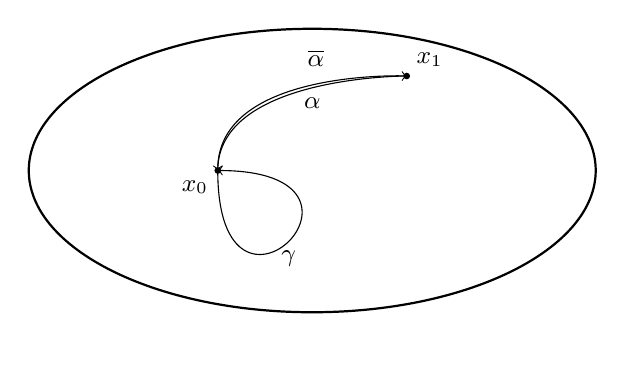
\begin{tikzpicture}[scale=1.2, every node/.style={font=\small}]
    % Draw the boundary of the space
    \draw[thick] (0,0) ellipse (3 and 1.5);

    % Points x0 and x1
    \fill (-1,0) circle (1pt) node[below left] {$x_0$};
    \fill (1,1) circle (1pt) node[above right] {$x_1$};

    % Path from x0 to x1
    \draw[->] (-1,0) .. controls (-1, 1) and (1, 1) .. (1, 1)
      node[midway, below] {$\alpha$};

    % Path from x1 to x0 (reversed)
    \draw[->] (1, 1) .. controls (1.1, 1) and (-1, 1.1) .. (-1, 0)
      node[midway, above=3pt] {$\overline{\alpha}$};

    % Loop \gamma at x0
    \draw[->] (-1, 0) .. controls (-1,-2) and (1,0) .. (-1, 0)
      node[midway, below] {$\gamma$};
  \end{tikzpicture}
\end{center}

\begin{proof}
  Define \( T_\alpha (\gamma) = \alpha * \gamma * \overline{\alpha} \).
  We show that \( T_\alpha \) is an isomorphism of groups.
  First,
  \begin{align*}
    T_\alpha(\varphi * \gamma) &= \alpha * \varphi * \gamma * \overline{\alpha} \\
                               &= \alpha * \varphi * \overline{\alpha} * \alpha * \gamma * \overline{\alpha} \\
                               &= T_\alpha(\varphi) * T_\alpha(\gamma)
  \end{align*}
  so \( T_\alpha \) is a group homomorphism.
  \( T_\alpha \) is bijective, since \( T_{\overline{\alpha}} \)
  is the inverse:
  \begin{align*}
    (T_{\overline{\alpha}} \circ T_{\alpha}) (\gamma)
      &= \overline{\alpha} * \alpha * \gamma * \overline{\alpha} * \alpha = \gamma \\
      (T_{\alpha} \circ T_{\overline{\alpha}}) (\gamma)
      &= \alpha * \overline{\alpha} * \gamma * \alpha * \overline{\alpha} = \gamma
  \end{align*}
\end{proof}
